The design and architecture described in the previous chapter is agnostic of the technology used for implementation. However, for evaluation and deployment of the state estimation to the race car, we are bound to the options offered by \gls{ecu} our \gls{vdc} software is running on, since the state estimation if part of that software, as described in section \ref{sec:design-computation-system}. We are using the ES910 produced by ETAS, which can connect to all \gls{can} buses for signal transport and runs code on top of a real-time operating system. Being a rapid prototyping module, the ES910 has significantly higher computing power with a floating-point processor and diagnostic interfaces~\cite[p.~16]{ETASGmbHStuttgart.2018}. Its software can be programmed with three technologies~\cites[p.~17]{ETASGmbHStuttgart.2018}[p.~10]{ETASGmbHStuttgart.2019}:
\begin{itemize}
\item ASCET: application development tool by ETAS, which generates safe C code from textual or visual models
\item MATLAB/Simulink: a model-based design tool by MathWorks, which generates C code
\item Custom code: write C code manually
\end{itemize}
While eventually the software will be transformed into C code, the model-based tools provide a convenient development experience, like visualization of signal flow, and safeguards against common errors. While both ASCET and MATLAB/Simulink are widely used, we decided on the latter option, since it is widely used for simulations and enables rapid testing of different approaches. More importantly, however, is the fact that the existing \gls{vdc} software is already developed in Simulink. Therefore, integration and build pipelines are already set up and integration is simple.


\section{Development}
Our basic building blocks for creating Simulink models are blocks, subsystems, referenced models, signals and buses. Best practices are described in the official modeling guidelines\cite{TheMathWorksInc..2020}, which we follow. Blocks are the basic functional unit, e.g., performing integration, boolean algebra, mathematical operations and input/output. They live in a model, which defines their execution context and is a single file. A special block is the MATLAB function, which can execute any MATLAB code that can be compiled to C code. Subsystems are a visual or functional group of blocks inside a model which cannot be reused. Other models can be referenced and thereby included in a model, facilitating reuse and collaboration because they are separate files. Signals are connections between blocks in the same model or across model boundaries. They can be grouped into buses, which simplify interface design for high-level components with many input/output signals.

The \gls{vdc} is a large Simulink model that includes the components shown in figure \ref{fig:architecture-integration} as referenced models, which means the state estimation is stored in a separate model file. Previously, a rudimentary state estimation without proper failure detection receives measurements and provided a state estimate for the subsequent components. Effectively, we replace this component while keeping the same interface, which enables drop-in replacement without the need for adaption of any other components.

We model the components of the state estimation as subsystems, since they are never reused and issues arising from collaboration, e.g., merge conflicts, are not a problem. Only components which are reused, such as the sanity check, are created as separate models and then referenced. While any algorithm and mathematical operation can be modeled using Simulink blocks alone, we use MATLAB code for the implementation of longer algorithms like the \gls{ekf} and \gls{imu} fusion but also many smaller operations. This approach proved to work well; Simulink acts as glue around the components which models signal flow, while MATLAB code is clearer when it comes to functionality and can easily be unit-tested easily in isolation. This separation of concerns makes the state estimation software clearer and more readable, another manifestation of our preference for simplicity.

We use strict bus definitions to describe the interface of components, including data types, dimensions and units. For example, there are buses for measurements from specific sensors, the total sensor state and the final estimate. While the definition of buses is development overhead, it helps to avoid logical errors like incorrect units that are rather hard to find and require manual troubleshooting. Furthermore, it helps to think of the components as black boxes with specified inputs and outputs, which then leads to the required functionality of the component. Single, short-lived signals inside of the components remain plain signals, however.

Previously, shared design data were stored in the MATLAB base workspace, which was set up by a parameter script. We migrated bus and parameter definitions as well as simulation configurations to data dictionaries, which are referenced from all models and submodels. This is the officially recommended way to store shared data, which makes it easy to track changes and control variable scope~\cite{TheMathWorksInc..2020b}.

Development comprised three major phases, following the three components shown in figure \ref{fig:architecture-stateestimation}. First, the preprocessing stage was implemented, which can be directly connected to the state estimate output, making isolated development of this stage possible. Next, we developed the \gls{ekf} responsible for sensor fusion, improving the measurements coming from the preprocessing stage. We also added a block to assemble the vehicle state bus by combining preprocessed data and the state estimate from the \gls{ekf}. Only in the last step, we implemented the outlier detection, determining the measurement mask for the \gls{ekf}. The final Simulink model for comparison with the designed architecture is shown in figure \ref{fig:simulink}. During each phase, the components were tested with recorded measurement data from the same sensors to guide design decisions. While testing the state estimation model in the context of the whole \gls{vdc} is possible, we created a separate model for development so we can test the state estimation in isolation. We were only able to perform model-in-the-loop testing, because the hardware required for hardware-in-the-loop testing was not available during development.

\begin{figure}
	\centering
	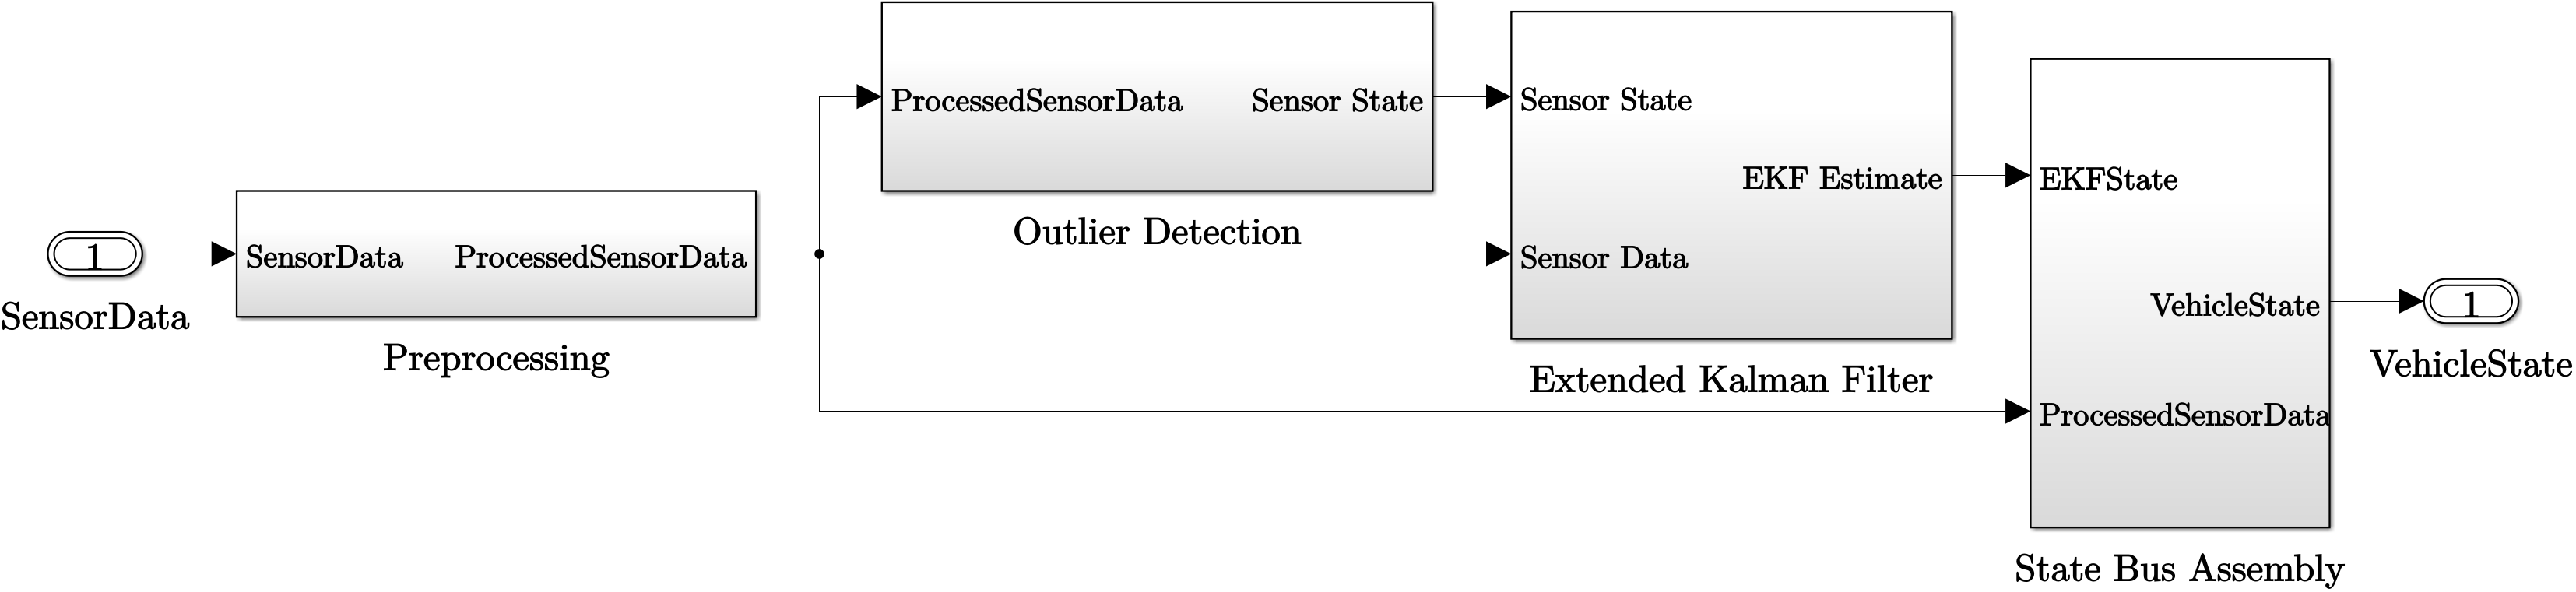
\includegraphics[width=\textwidth]{simulink}%
	\caption{Implementation as Simulink model}
	\label{fig:simulink}
\end{figure}


\section{Deployment}
During development, the state estimation model can easily be executed on the development computer. However, deploying the Simulink model to the ES910 platform requires a series of steps, shown in figure \ref{fig:build-toolchain}.

\begin{description}
\item[Code Generation] The first step is to generate C code from the Simulink model and included MATLAB code using Simulink Coder with an specific target, adjusting code generation to the requirements of the ES910. The generated code includes a step function to execute one iteration of the model. Additionally to the code, a module and interface description is generated. Note that Simulink Coder does not support all language features, so some code might need to be restructured for code generation.

\item[Integration] ETAS' INTECRIO is used to integrate the generated code module into the ES910 system based on the module description. This includes scheduling the \gls{vdc} for execution every \SI{1}{\milli\second} and connecting \gls{can} signals to their respective model inputs and outputs. INTECRIO builds all modules into an executable file and a file describing calibration and measurement variables.

\item[Installation] The executable file can be transferred to the ES910 and flashed onto its memory using ETAS' INCA. Once the ES910 is started, INCA can also be used to monitor signals, both internal in the software and external coming from the \gls{can}, and control parameters.
\end{description}

\begin{figure}
	\centering
	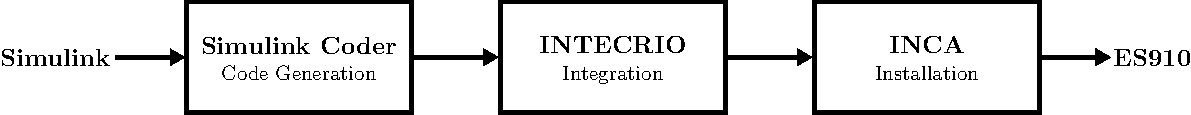
\includegraphics[width=\textwidth]{build_toolchain}%
	\caption{Build and deployment toolchain}
	\label{fig:build-toolchain}
\end{figure}

Once the state estimation is deployed to the ES910 and connected to all sensors in the vehicle, it can be calibrated and tuned to the hardware. This includes adjustment of the failure detection thresholds, \gls{imu} rotation correction and \gls{ekf} measurement covariance settings.
